% preamble
\documentclass[preprint, 3p, times, compress, 11pt]{elsarticle}
\usepackage{lineno, amsmath, float, graphicx, subfigure, color, multirow, 
        algorithm, algpseudocode, setspace, caption, hyperref, booktabs} 
\graphicspath{{res/}, {res/bridge/}, {res/classify/}, {res/deri/}, 
        {res/flowchart/}, {res/software/data/}} 
\captionsetup[figure]{labelfont={bf}, name={Fig.}, labelsep=period}
\captionsetup[table]{labelfont={bf}, name={Table}, labelsep=space}
\captionsetup[algorithm]{labelfont={bf}, name={Algorithm}, labelsep=period}
\renewcommand{\algorithmicrequire}{\textbf{Input:}}
\renewcommand{\algorithmicensure}{\textbf{Output:}}
\newcommand{\tabincell}[2]{\begin{tabular}{@{}#1@{}}#2\end{tabular}}
% \modulolinenumbers[5]
\linenumbers
\journal{MEASUREMENT}
\bibliographystyle{elsarticle-num}

% document
\begin{document}

% front matter
\begin{frontmatter}
% title
\title{Identification of Intense Vortex-induced Vibration on Bridge Cables 
        Applying Dynamic Indicators and Probability-based Partitioning}
% author
\author[tongji]{Jinghang Weng}
\author[tongji]{Lin Chen\corref{correspond}}
\ead{linchen@tongji.edu.cn}
\author[tongji,lab,qizhi]{Limin Sun\corref{correspond}}
\cortext[correspond]{Corresponding author. Department of Bridge Engineering, 
    Tongji University, 1239 Siping Road, Shanghai 200092, China}
% affiliation
\address[tongji]{Department of Bridge Engineering, Tongji University, 
    Shanghai 200092, China}
\address[lab]{State Key Laboratory of Disaster Reduction of Civil 
    Engineering, Tongji University, Shanghai 200092, China}
\address[qizhi]{Shanghai Qi Zhi Institute, Shanghai 200092, China}

% abstract
\begin{abstract}
Vortex-induced vibration (VIV) is one of the most common anomalous 
oscillations faced by cables on cable-stayed bridges, suspension bridges
and arch bridges. Typically, cable VIV is a kind of abnormal vibration 
with large displacements and thus imposes detrimental implications 
on cables and even the whole bridge structure. Therefore, this study 
designs an efficient method to spontaneously recognize intense VIV 
and send instant warnings. While the root mean square of acceleration 
represents the intensity of vibration, another indicator deriving from 
derivation transform is designed to quantify the degree of single-mode 
vibration. Comparing with other equivalent coefficients, this indicator 
can be easily calculated and is free from the interference of end effect, 
thus enhance both the efficiency and accuracy. Subsequently, the two 
dynamic indicators, after several algebraic transformations, are utilized 
together to create a mixed feature (MF). Given a certain threshold, a 
probability-based partitioning strategy considering the distribution 
of MF is introduced to extract VIV samples from all the vibration samples, 
hence consolidating the foundation of multi-level intense VIV warning. 
The proposed method has been validated in VIV identification of cables on 
a large-span cable-stayed bridge. The dynamic features of cables both
frequently and hardly influenced by VIV are compared and discussed. 
\end{abstract}

\begin{keyword}
Bridge cable \sep Vortex-induced vibration \sep Derivation transform \sep 
Dynamic indicator \sep Probability-based partitioning \sep Instant warning. 
\end{keyword}
\end{frontmatter}

% main body
\section{Introduction}

Known for its frequent occurrence in cable-stayed bridges and suspension 
bridges, vortex-induced vibration (VIV) usually brings about large cable 
displacement and follows irrevocable detrimental influences. Therefore, 
it is essential to conceive an efficacious method that can spontaneously 
recognize VIV and send instant warnings. Generated by vortices 
periodically separating from either side of a bluff body when fluid 
passes it, the force that causes VIV is represented by a non-dimensional 
number, i.e., the Strouhal number, which can be calculated by 

\begin{equation}
    St = \frac{fD}{U},
    \label{eq:Strouhal}
\end{equation}

where $St$ is the Strouhal number and $f$, $D$ and $U$ refer to the 
frequency of the airflow, the diameter of a bridge 
cable, and the speed of the airflow, respectively \cite{jafari2020windinduced}. 

Traditionally, three major methods are frequently utilized to explore 
the characteristics of VIV, i.e., theoretical analyses, computational fluid 
dynamics simulations, and wind tunnel tests. Nevertheless, the mechanism 
underlying VIV is still uncovered due to the high nonlinearity of 
airflow and cable-fluid interaction. Nowadays, the prevalence of 
structural health monitoring (SHM) system offers a tremendous 
opportunity for the big-data-based study of cable vibration. Due to 
their convenience and relatively low price, accelerometers are widely 
deployed in SHM systems as the major data resources. The root mean square 
(RMS) of acceleration time history is then deemed as the prime indicator 
to quantify the cable vibration intensity. However, more information is 
desired to distinguish VIV from other anomalies with intense oscillations. 

\textcolor{red}{
    ref: why intense VIV is single-mode
}

Typically, researchers employed the Fourier transform to obtain either 
the frequency spectrum or power spectrum, which can be used to analyze 
the excited modes. The spectrum with a single high peak indicates the 
occurrence of VIV since this kind of vibration usually comprises only 
one major vibration frequency \cite{li2018datadriven}. 
Recently, scholars presented several innovative methods to detect VIV 
from acceleration time history. Huang, Z. et al. \cite{huang2019automatic} 
employs Random Decrement Method to deepen the difference between VIV 
and normal ambient vibration, thus making it more precise for VIV 
identification. To automatically sieve out the non-stationary section of 
the so-called abnormal vibration, i.e., the VIV, Zhao, H. et al. 
\cite{zhao2022statemonitoring} takes advantage of Gaussian mixture 
modeling of the envelope of time history. After that, the stationary 
section is selected to extract modal parameters. Among all these methods, 
the novel algorithm based on the Hilbert transform (HT) 
is one of the most prevalent. A composite complex analytic signal, whose 
real part is the original signal while the imaginary part represents the 
HT of the original, is introduced into this method. The projection of 
such a signal on the complex plain reflects the constituent of the 
vibration, as Dan, D. and Li, H. \cite{dan2022monitoring} suggest, the 
more it resembles a hollow ring, the more remarkable its single-mode feature, 
and thus the more exact the occurrence of vortex-induced vibration. 
Although the method that employs HT is precise, it is somewhat 
time-consuming, since based on the Fast Fourier transform, whose time 
complexity is O(nlogn). To enhance the time efficiency, this paper 
proposes a derivative indicator based on discrete numerical 
differentiation, which has an O(n) time complexity, thus obviously 
lowering the calculative time and bringing about a dependable on-time warning. 

Furthermore, since any individual indicator merely denotes either the 
intensity or the degree of single-mode, more than one indicator should 
be analyzed for the identification of intense VIV. 
He, M. et al. \cite{he2022online} 
present two indicators based on the power spectrum and HT analytical 
signal respectively. These two indicators are then employed to 
differentiate VIV and normal vibration based on a pre-set line that 
relies on practical experience. In addition to that, multifarious 
clustering algorithms are introduced to achieve unsupervised 
classification. He, M. et al. \cite{he2022identification} claim that 
KMeans might be the best choice to separate different kinds of vibrations 
since both hierarchical and density-based clustering entail some 
hyper-parameters that could not be precisely determined. Li, S. et al. 
\cite{li2017cluster}, however, use a novel clustering strategy deriving 
from the traditional density-based algorithm to detect the VIV in the 
beam of a suspension bridge. Nevertheless, KMeans applied by He, M. et al. 
\cite{he2022identification} is extremely sensitive to outliers, while the method 
employed by Li, S. et al. \cite{li2017cluster} demands laborious analysis 
when determining the number of cluster centroids. To overcome these 
shortages, a method applying the DBSCAN clustering algorithm is used 
in discriminating different vibrations based on RMS and the derivative 
indicator, i.e., the hollow coefficient of the derivative analytical 
signal (HCD). SHM data of a long-span cable-stayed bridge are analyzed 
accordingly, and the result proves both the accuracy and efficiency of 
such a method.

The remaining sections are organized as follows. The methodology of VIV 
identification is explicated in Sec.~\ref{sec:method}, where two indicators 
together with a probability-based partitioning strategy are introduced. 
In Sec.~\ref{sec:experiment}, these methods are carried out to identify 
the VIV occurring in cables on a long-span cable-stayed bridge, whose 
SHM system has recorded the long-time acceleration time history of several
cables. Finally, conclusions are drawn in Sec.~\ref{sec:conclusion}.

\section{Automated cable VIV identification method}
\label{sec:method}

\subsection{Key indicators to represent vibration features} 
  

\subsubsection{RMS to indicate the intensity of vibration}

When VIV occurs on a cable, its vibration is usually much more intense 
than in normal circumstances. Therefore, the RMS of a piece of 
acceleration time history $\{a_i\}$ is applied to represent the intensity 
of cable vibration, which can be calculated by 

\begin{equation}
    RMS = \sqrt{\frac{1}{N} \sum_{i=1}^{N} a_{i}^{2}},
    \label{eq:RMS}
\end{equation}

where $N$ is the length of the time series. Generally, the larger the RMS, 
the more likely a certain kind of abnormal vibration is to occur.

\subsubsection{Indicators to quantify the single-mode characteristic}

% Peak ratio of spectrum

% Hollow coefficient of Hilbert analytical signal

The RMS, though a helpful indicator to suggest the presence of abnormal 
vibration, purveys no additional information to discriminate VIV from other 
large-amplitude abnormal vibrations. Therefore, the single-modal property 
of large-amplitude VIV is taken into consideration by applying HT, 
which is demonstrated by 

\begin{equation}
    y(t) = x(t) * \frac{1}{\pi t} = \int_{-\infty}^{+\infty} 
            \frac{x(\tau)}{\pi(t-\tau)} dt, 
    \label{eq:hilb}
\end{equation}

where $y(t)$ and $x(t)$ represent the transformed signal and the 
original signal, respectively. 

The Hilbert analytical signal is then defined as a complex signal 

\begin{equation}
    z(t) = x(t) + iy(t),
    \label{eq:comp_sign}
\end{equation}

which consists of both the original 
signal $x(t)$ and the transformed signal $y(t)$. 

It is mathematically proved that the HT of a sine function is its 
corresponding cosine function and vice versa. According to this feature, 
if a cable is under an ideal VIV situation, i.e., the original acceleration 
signal is a sine function, the projection of its Hilbert analytical 
signal in the complex plane will be a circle (see Fig.~\ref{fig:proj_hilb}~(a), 
where all the physical quantities are normalized in advance). Practically, 
due to the broadband components of the force caused by the vortex and the 
influence of environmental noises, the projection of the analytical 
signal is a ring with an inner radius R1 and outer radius R2, as shown 
in Fig.~\ref{fig:proj_hilb}~(b).

\begin{figure}[ht]
    \centering
    \subfigure[Ideal sine function]{
        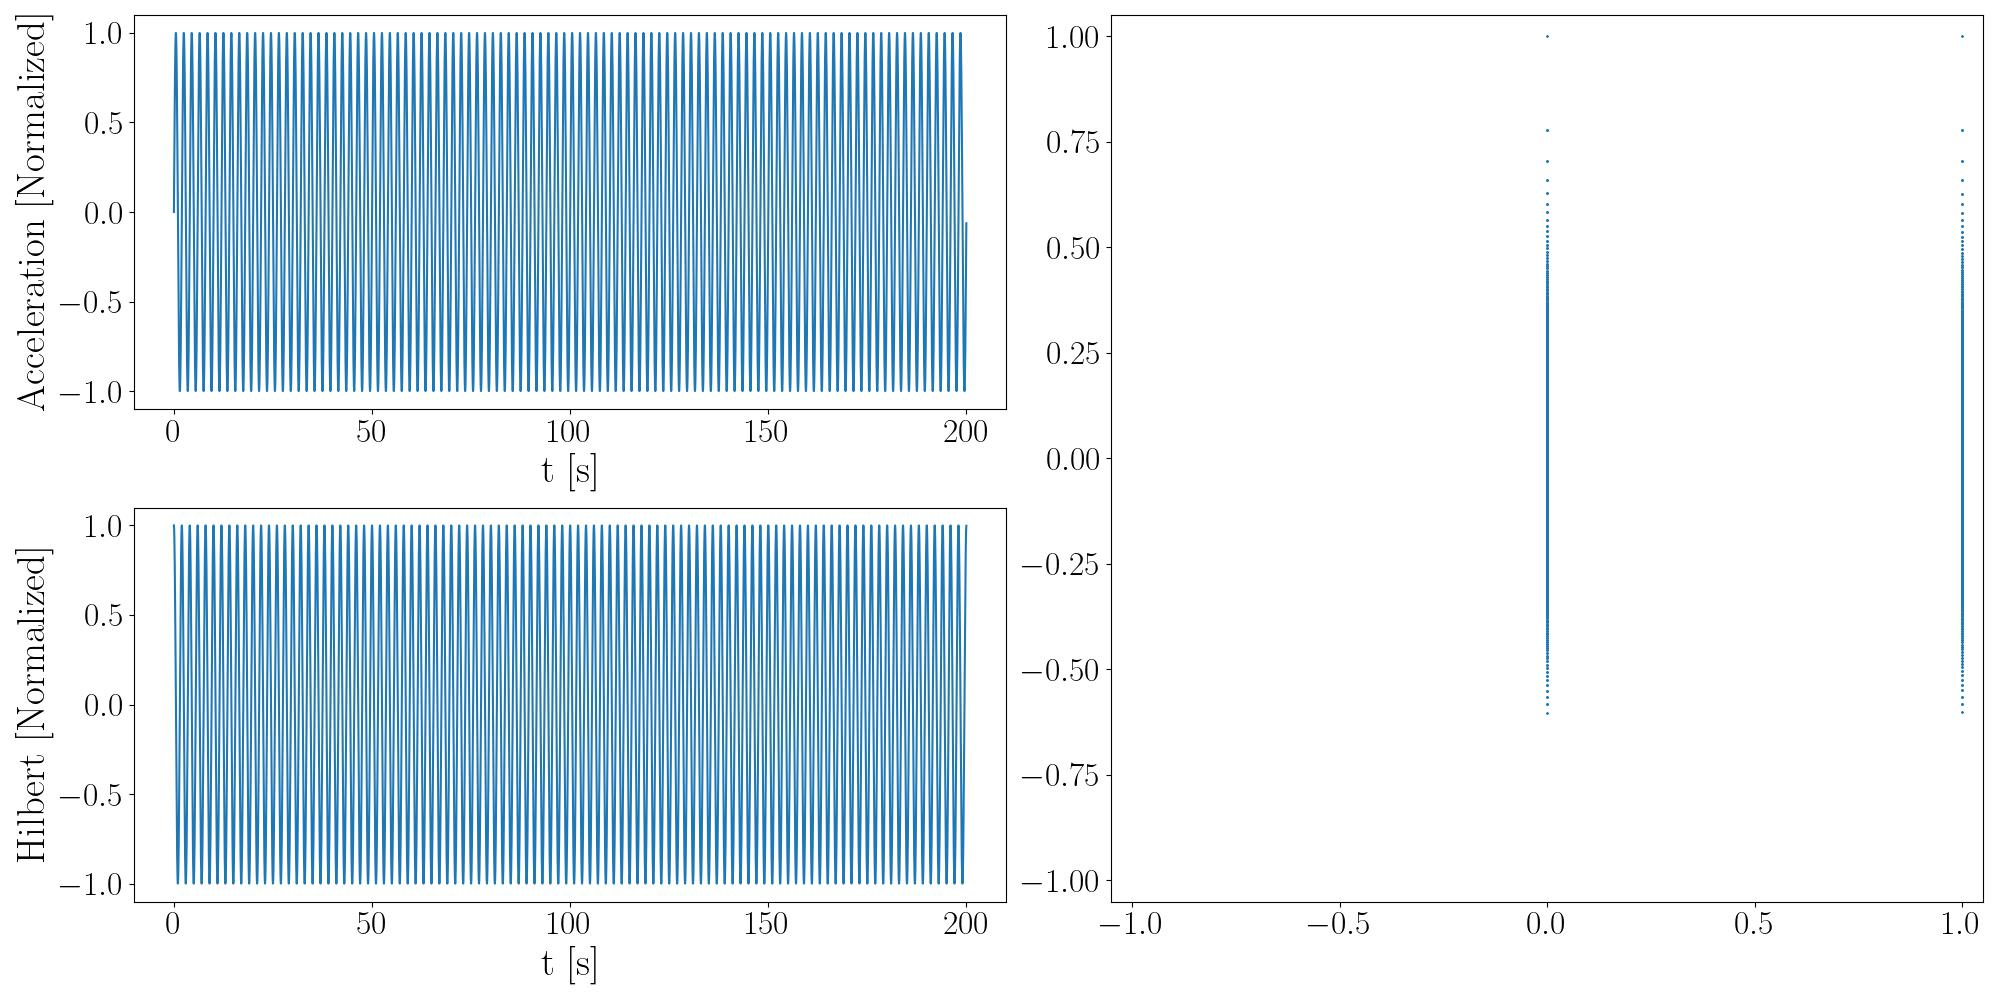
\includegraphics[width=0.8\textwidth]{hilbert_ideal_sin.jpg} 
    }
    \qquad
    \subfigure[sine function with noises]{
        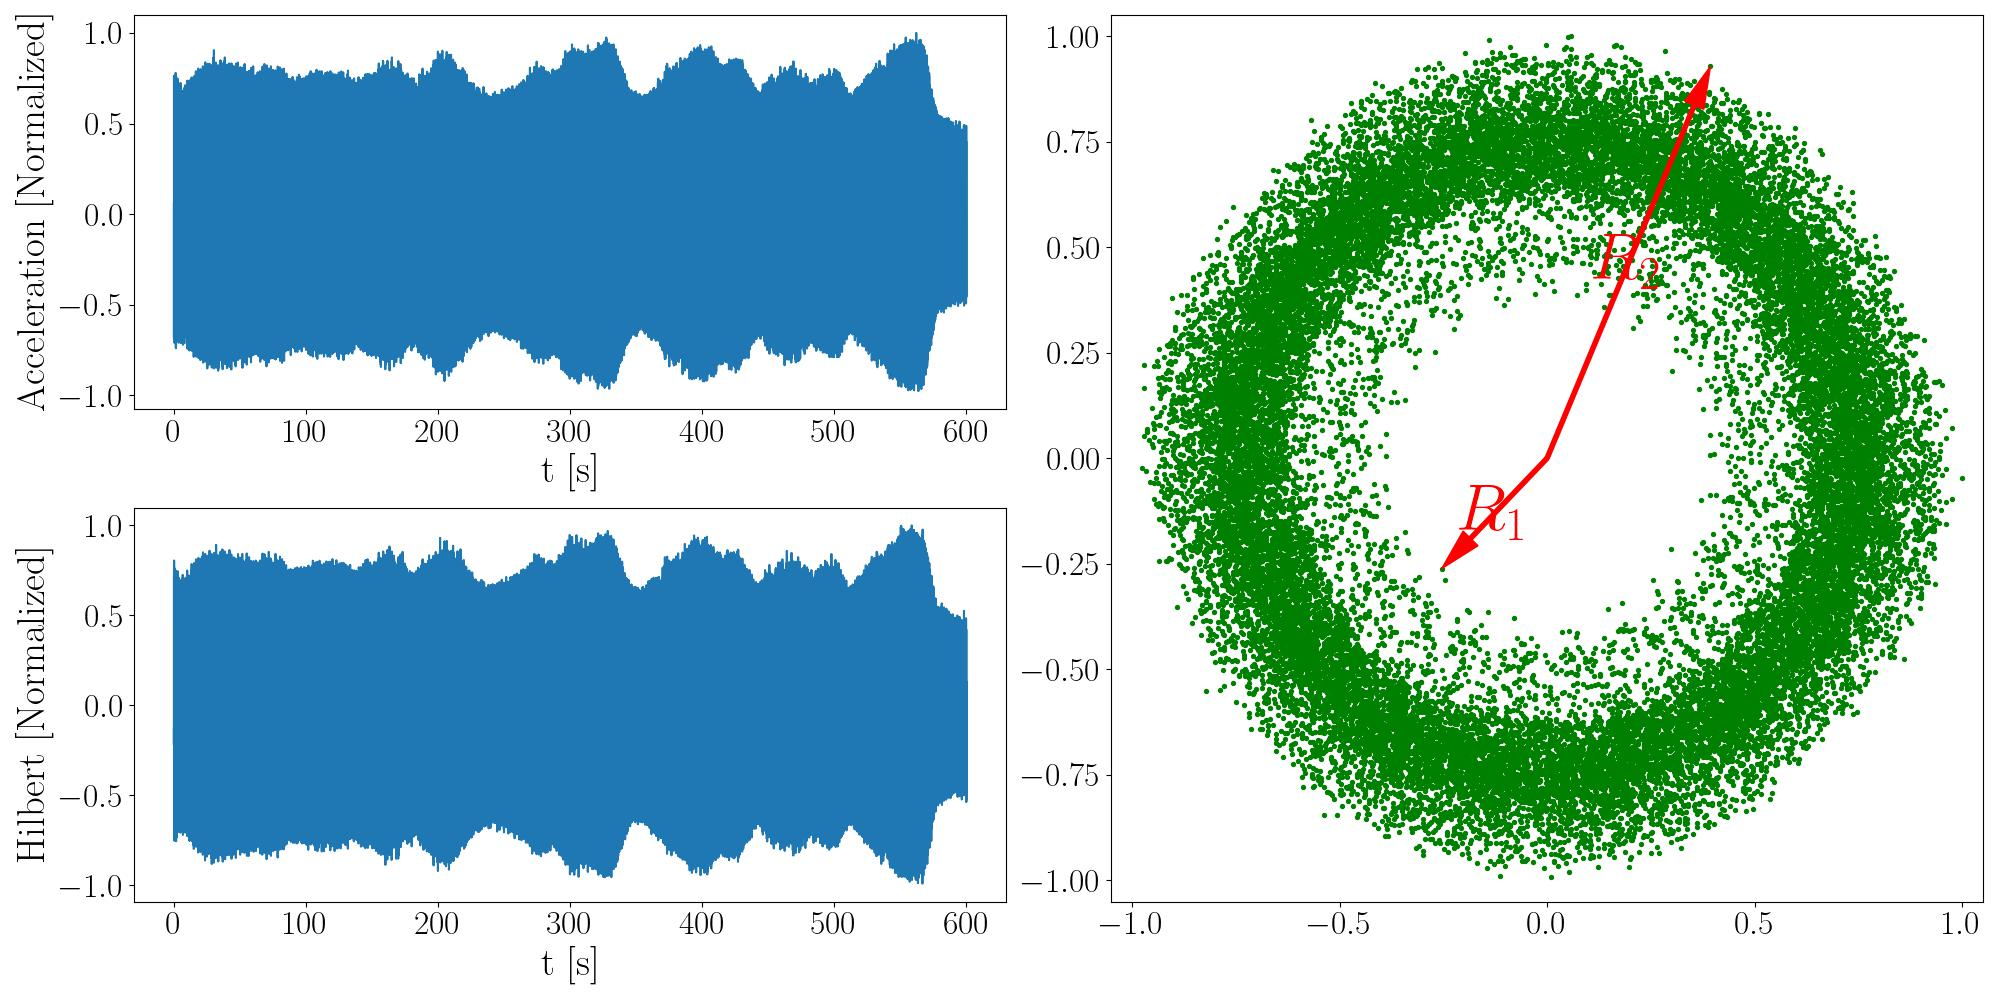
\includegraphics[width=0.8\textwidth]{hilbert_real_sin.jpg}
    }
    \caption{Projection of the Hilbert analytical signal of a sine 
            function in a complex plain.}
    \label{fig:proj_hilb}
\end{figure}

To quantify the single-modal feature of VIV, the HCH is defined by 

\begin{equation}
    HCH = \frac{R_1}{R_2},
    \label{eq:HCH}
\end{equation}

where $R1$ and $R2$ represent the inner radius and outer radius 
displayed in Fig.~\ref{fig:proj_hilb}~(b).

It is understandable that the more the HCH is closer to one, the more 
similar the ring is to a circle, and thus the more obvious the emergence 
of single modal vibration is. 

% Hollow coefficient of Derivative analytical signal

The analytical signal applying the signal transformed by HT as the 
imaginary part is indeed useful. Despite that, the long time it spent 
due to the O(nlogn) time complexity of HT makes it difficult for in-time 
detection and warning. To cope with this predicament, the Derivative 
Transform (DT) is defined as 

\begin{equation}
    \left \{
        \begin{aligned} 
            &\hat{y}(t) = \frac{dx(t)}{dt}, \\ 
            &y(t) = \frac{\hat{y}(t)}{max \left( \hat{y}(t) \right)},
        \end{aligned} 
    \right. 
    \label{eq:deri}
\end{equation}

which is designed to substitute the HT, while the composite complex 
signal can still be represented by Eq.~\eqref{eq:comp_sign}.

Overall, such a substitution reduces the time complexity to O(n), which 
descends from the calculative expense of the numerical differentiation 
of a time series. The feasibility of this replacement relies on the 
fact that the derivative of a sine function is a cosine function and 
vice versa. Moreover, one additional matter worth attention is that 
the new signal derived from the derivative transform should be normalized 
one more time since this process introduces a multiplier $\omega$, which 
is the circular frequency of a sine or cosine function. 

Similarly, the projection of the derivative analytical signal of the sine 
function in a complex plain is shown in Fig 2., where Fig.~\ref{fig:proj_deri}~(a) 
and Fig.~\ref{fig:proj_deri}~(b) represent the ideal condition and 
noise-influenced condition, respectively. HCD is correspondingly defined as 

\begin{equation}
    HCD = \frac{R_1}{R_2},
    \label{eq:HCD}
\end{equation}

whose variables have identical meanings to those in Eq.~\eqref{eq:HCH}.

\begin{figure}[ht]
    \centering
    \subfigure[Ideal sine function]{
        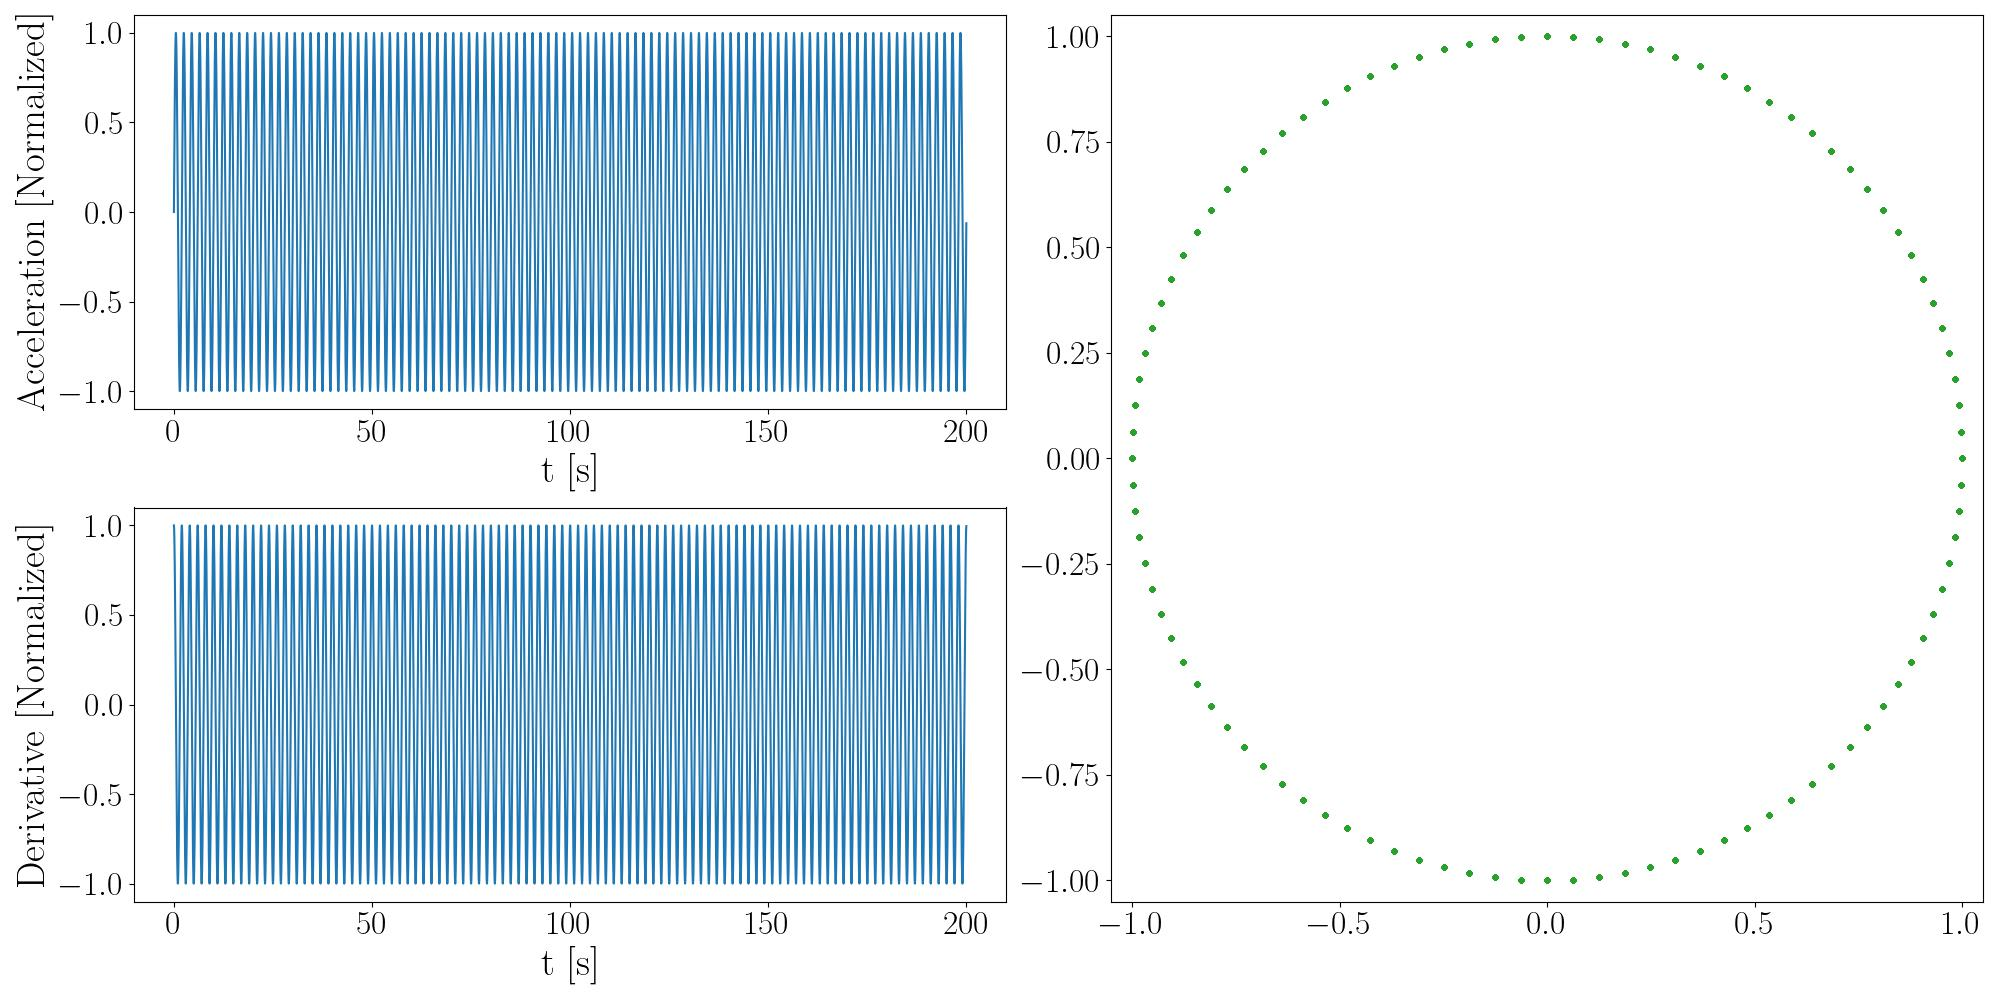
\includegraphics[width=0.8\textwidth]{derivative_ideal_sin.jpg} 
    }
    \qquad
    \subfigure[sine function with noises]{
        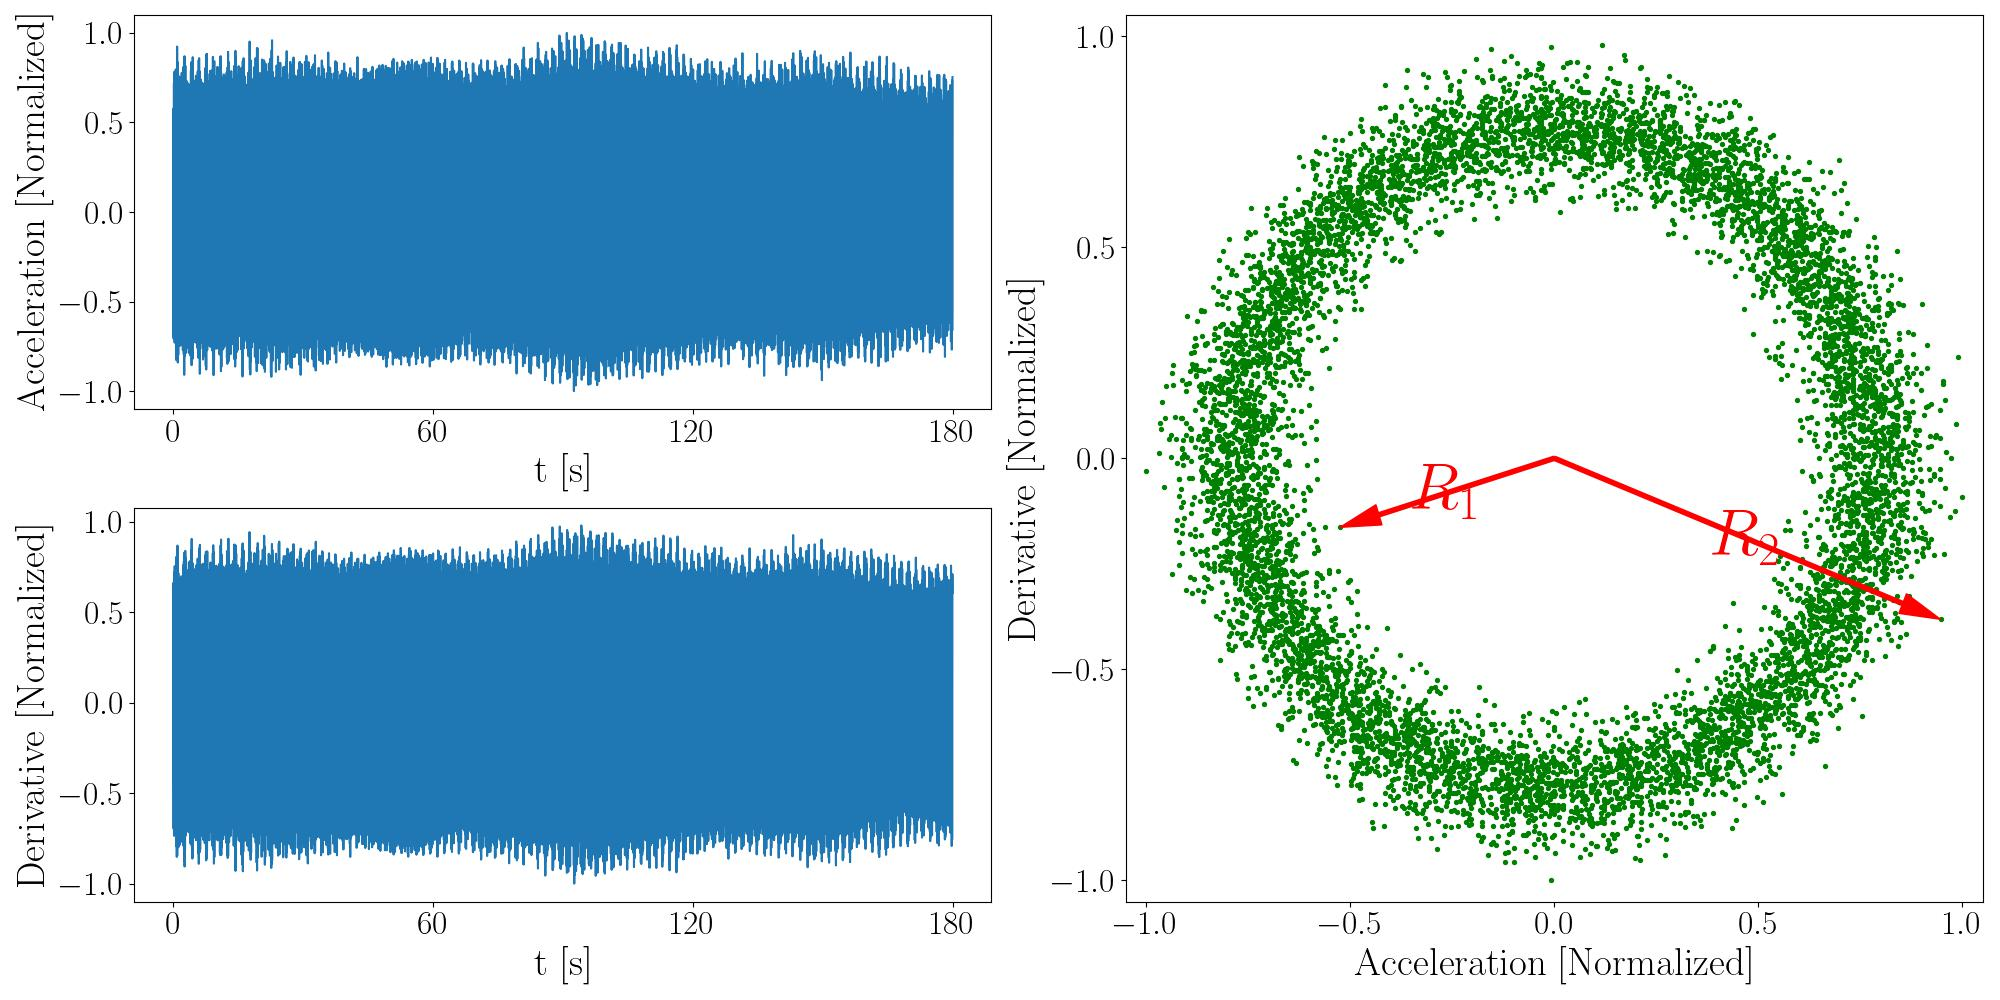
\includegraphics[width=0.8\textwidth]{derivative_real_sin.jpg}
    }
    \caption{Projection of the Derivative analytical signal of the sine 
            function in a complex plain.}
    \label{fig:proj_deri}
\end{figure}

\textcolor{red}{
    merits: O(n), no end effect, circular queue
}

\subsection{Sample classification based on probability distribution and 
        outlier threshold}

\textcolor{red}{
    why lower convex function?
    flowchart!
}

\subsubsection{Typical distribution of RMS and HCD}

\subsubsection{Logarithm transformation of RMS and HCD to extend data 
        distribution}

\subsubsection{Mixed Feature of TRMS and THCD}

\textcolor{red}{
    1. PCD
    if cannot PCD, usually not VIV 
    2. distribution
}

\subsubsection{Sample partitioning according to the distribution of the 
        mixed feature}

\subsubsection{Probability-based boundary curve in the RMS-HCD plain}

\textcolor{red}{
    lots of math...
}

\subsection{Multi-level VIV warning applying RMS and HCD}

\subsubsection{VIV warning with several probability thresholds}

\subsubsection{VIV warning considering the abstract values of RMS and HCD}

\section{Application to a long-span cable-stayed bridge}
\label{sec:experiment}

\subsection{Description of the Tongling Yangtze River Bridge and its SHM system}

The methods and algorithms proposed in Sec.~\ref{sec:method} are 
applied for cable VIV identification of the Tongling Yangtze River 
(TYR) Bridge. Locating in Tongling City, Anhui province, China, the TYR bridge 
is a long-span cable-stayed bridge, whose cables intermittently suffer 
from VIV. Therefore, this research might help the bridge owner to 
detect VIV and send instant warnings.

One cable in the TYR Bridge, which is attached to an accelerometer 
named ACC-C01-01, is applied to explicate the whole process. The original 
data provided by SHM system is the time history of acceleration within an 
hour, whose file type is MATLAB's mat file. First of all, the one-hour 
continuous time history is divided into several pieces by a time window 
with a length of 10 minutes and a slide step of 5 minutes, and the RMS 
of each time interval is calculated. Then, the Fast Fourier Transform 
follows to secure the frequency spectrum of acceleration. Furthermore, 
both the HT and the derivative transform are performed respectively to 
get the HCH and HCD. Finally, all the indicators, i.e., the RMS, HCH, 
and HCD are considered together by KMeans and DBSCAN to classify VIV and 
normal vibration. 

\subsection{Sample acquisition and feature analysis}

\subsubsection{Data Processing and parameter setting}

\subsubsection{Statistical analysis to attest the equivalence of HCH and HCD}

Fig.~\ref{fig:time_freq_hilb_deri} indicates not only that the 
projections of the two analytical signals during VIV are distinct from 
that during non-VIV conditions, but that the two are almost identical 
when dealing with the same period of a signal. On the one hand, 
projections during the non-VIV are similar solid circles. On the other 
hand, those during the VIV are similar hollow rings with approximately 
equal inner radii and outer radii.

To further confirm the identity of the derivative transform and HT when 
recognizing VIV, Fig.~\ref{fig:HCH_HCD} plots all the samples into an 
HCD-HCH coordinate system, where all the scatter points almost distribute 
in the line $HCD = HCH$, which means these two indicators offer 
the same information to detect the single modality. 
Therefore, it is reasonable to replace 
the complicated HT with the much more efficient derivative transform. 
Another matter that demands attention is that all the normal vibration 
samples have an almost zero-value HCD and an almost zero-value HCH, 
making themselves concentrated in the coordinate origin and covered by 
some VIV sample points.

\begin{figure}[ht]
    \centering
    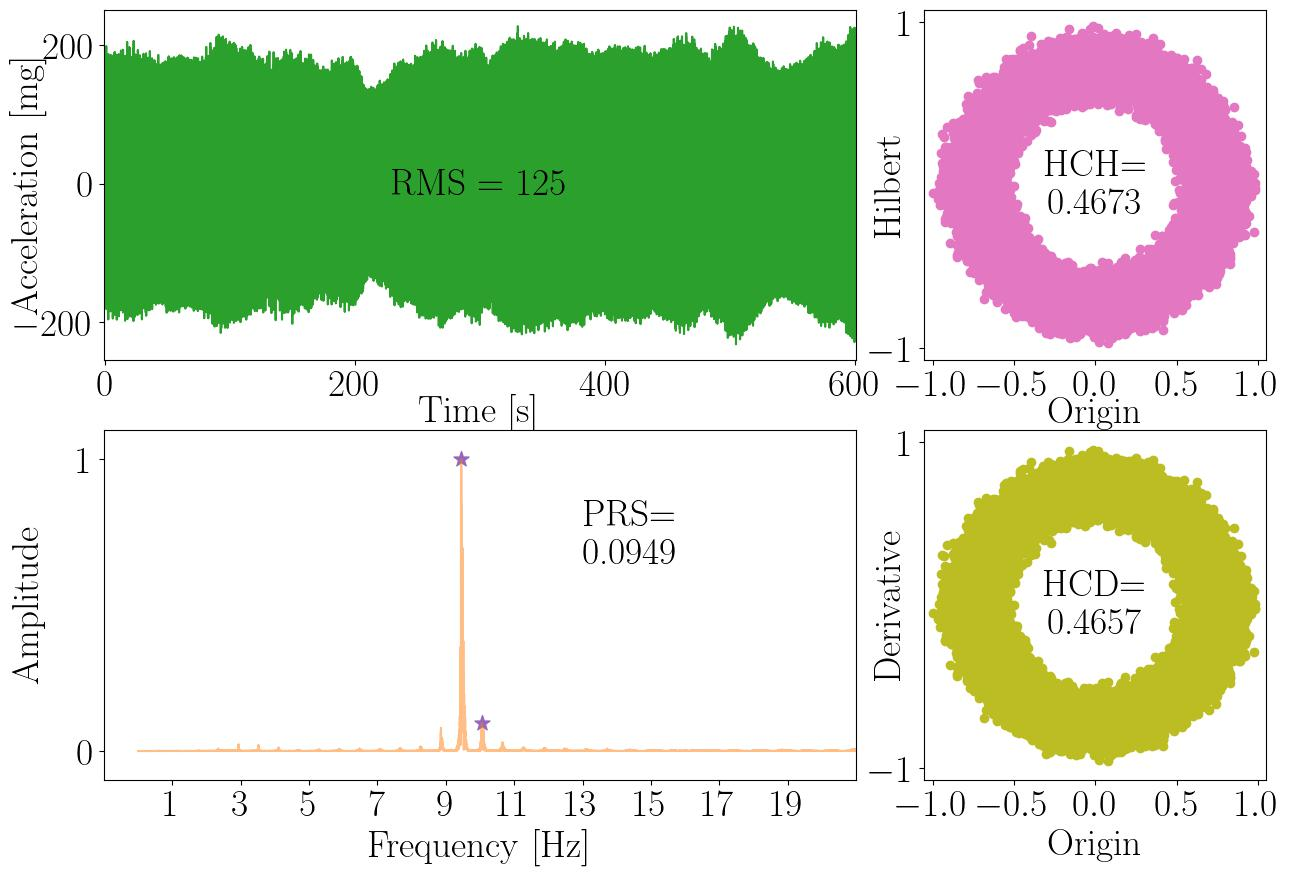
\includegraphics[width=0.64\textwidth]{viv.jpg}
    \caption{Scatter diagram to compare HCH and HCD.}
    \label{fig:HCH_HCD}
\end{figure}

\subsection{Illustration of typical VIV and non-VIV} 

As mentioned above, each one-hour continuous time history is sliced by 
a ten-minute time window. It is noteworthy that since the slide step of 
this time window is five minutes, there is a five-minute overlapping 
region between each two contiguous time windows. As a result, each 
one-hour raw data offers eleven samples.

The discrepancy between VIV and normal vibration is remarkable. 
Fig.~\ref{fig:time_freq_hilb_deri} shows the ten-minute time history, 
frequency spectrum, and projections of both the Hilbert analytical signal 
proposed by Dan, D. et al. \cite{dan2022monitoring} and the 
derivative analytical signal. It is noticeable that the RMS of VIV is 
much bigger than that in normal vibration. Moreover, the frequency 
spectrum of acceleration during VIV almost merely comprise one 
eigenfrequency, while that during normal condition contains multiple 
modal components. What's more noticeable, both the projections of the 
Hilbert analytical signal and derivative analytical signal display a 
hollow ring and solid circle in VIV and non-VIV circumstant, 
respectively. In a nutshell, the VIV manifests a strong attribution 
of large amplitude and approximately unimodal vibration.

\begin{figure}[ht]
    \centering
    \subfigure[Normal ambient vibration]{
        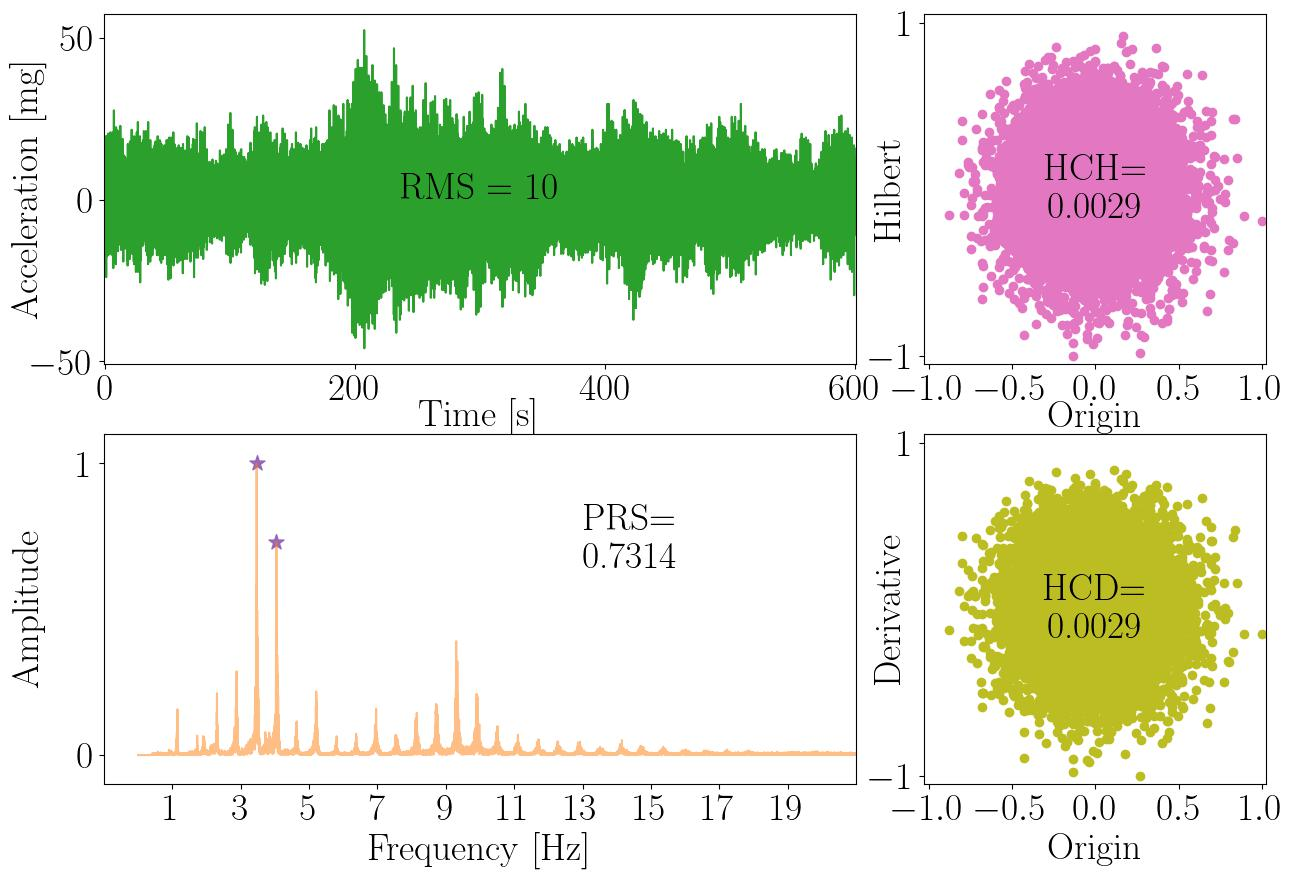
\includegraphics[width=0.8\textwidth]{normal.jpg} 
    }
    \qquad
    \subfigure[VIV]{
        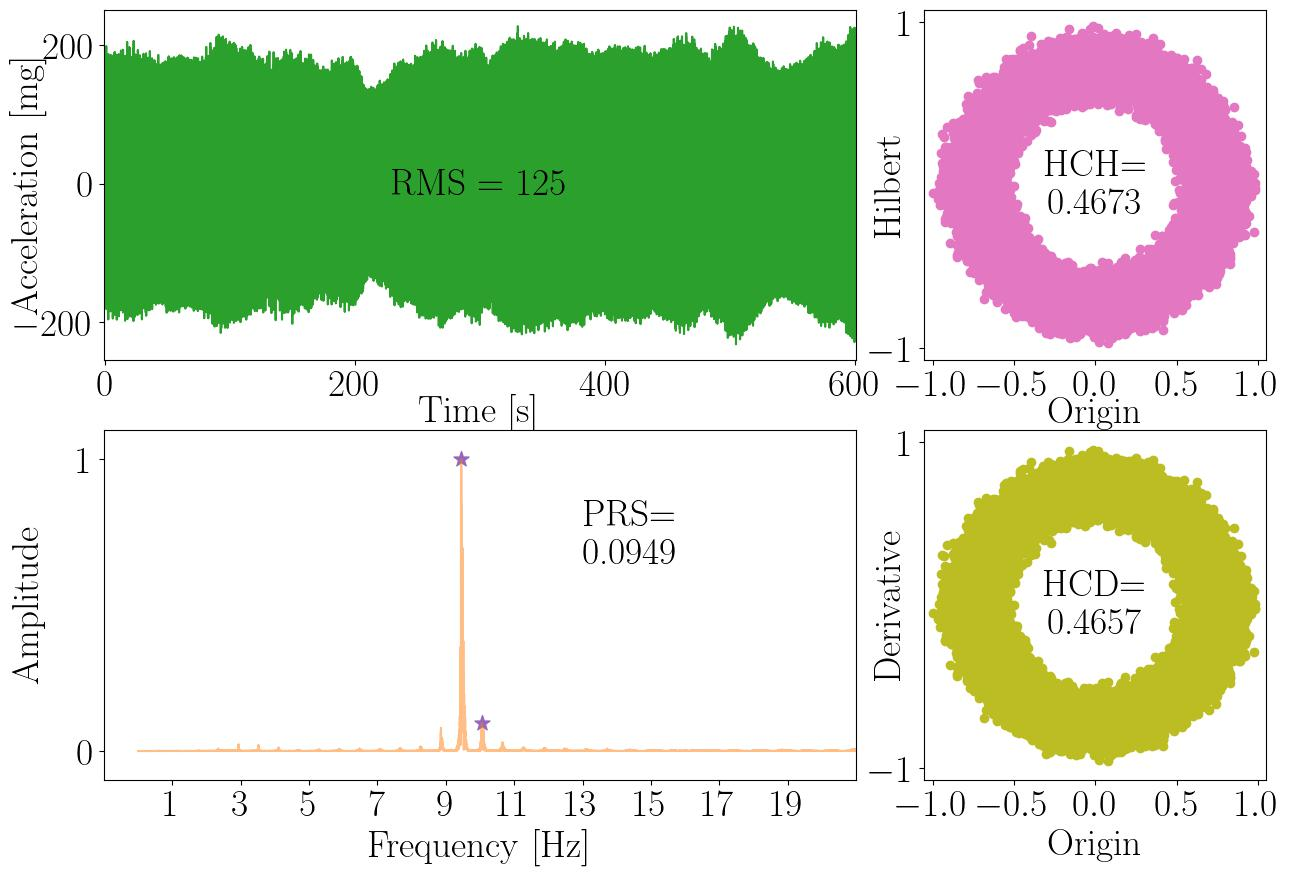
\includegraphics[width=0.8\textwidth]{viv.jpg}
    }
    \caption{Time history, frequency spectrum, projections of the two 
            analytical signals in an hour.}
    \label{fig:time_freq_hilb_deri}
\end{figure}

\subsection{Recognition of intense VIV on different cables}

\subsubsection{Cables with massive intense vibration sampels}

\subsubsection{Cables with almost no intense vibration samples}

\subsection{Parametric analysis}

\subsubsection{Order coefficient in the logarithm transformation}

\subsubsection{Thresholds for sample classification}

\clearpage

\section{Conclusions}
\label{sec:conclusion}

To detect the occurrence of VIV in bridge cable, two key indicators, i.e., 
the RMS and HCH, is utilized to extract certain feature from acceleration 
time history. Drawn in the HCD-RMS coordinate system, the vibration sample 
points can be divided into two classes by two clustering algorithms 
automatically. The proposed methods make it possible to achieve real-time 
warning of VIV in the future and the following conclusions can be drawn.

\begin{enumerate}[(1)]
    \item 
RMS and HCH demonstrate high accuracy to quantify the intensity 
and mono-modality of a period of vibration. While offering nearly the 
same information compared with the HCH, the HCD is much more efficient 
since it is based on the derivative transform, whose time complexity is O(n).
    \item
Probability-based classification is much more precise compared with that 
depending on the KMeans.
    \item 
The method is based on past data and thus highly contingent on the specific 
environment.
\end{enumerate}

% invoke
\bibliography{VIV}
\end{document}
